\documentclass[11pt,a4paper]{article}
\usepackage[all]{xy}
\usepackage{amsmath, amssymb}
\usepackage{algorithm, algorithmicx, algpseudocode}
\usepackage{stmaryrd}
\usepackage{color}
\usepackage{graphicx}
\usepackage[utf8]{inputenc}
\usepackage{hyperref}
\usepackage{url} %Shouldn't be needed
\usepackage{tikz}
\usepackage{booktabs}
\usetikzlibrary{arrows, automata, positioning}
%\usepackage[natbibapa]{apacite}

%Settings
\hypersetup{
	colorlinks=false,
	bookmarks=true,
	linkcolor=blue
}
\graphicspath{{./Pics/}}
\numberwithin{figure}{section}
\bibliographystyle{plain}

%\usepackage[rightcaption]{sidecap}
%\usepackage{float}

%Commands
\newcommand{\todo}[1]{\textcolor{cyan}{(TODO: #1)}}
\newcommand{\question}[1]{\textcolor{red}{(ASK TRULS: #1)}}
\newcommand{\bisim}{\mathfrak{R}}

%Commonly used variables
\newcommand{\states}{S}
\newcommand{\rels}{\sim}
\newcommand{\ags}{A}
\newcommand{\vals}{V}
\newcommand{\props}{P}
\newcommand{\model}[1]{$M#1 = (\states#1, \rels#1, \vals#1)$}
\newcommand{\lang}[1]{$\mathcal{L}_{#1}$}
\newcommand{\M}{\mathcal{M}}
\newcommand{\dia}[1]{\langle#1\rangle}
\newcommand{\eqc}[1]{\llbracket#1\rrbracket}
\newcommand{\ext}[1]{||#1||}
\newcommand{\labels}[1]{F_{#1}}
\newcommand{\anns}[1]{\mathcal{A}_{#1}}
\newcommand{\cname}{GALMC}

%Enviroments
\newtheorem{thm}{Theorem}[section]
\newtheorem{cor}[thm]{Corollary}
\newtheorem{lem}[thm]{Lemma}
\newtheorem{conjecture}[thm]{Conjecture}
\newtheorem{definition}[thm]{Definition} %Make definitions start on new line?
\newtheorem{proposition}[thm]{Proposition}
\newtheorem{example}[thm]{Example}
\newtheorem{fig}{Figure}[section]

\begin{document}

%\author{Anders Eide}
%\title{To be announced: \\\large Understanding and model checking Group Announcement Logic}
%\date{Sometime in the future}
%
%\maketitle
%\question{Hvordan pynte dette?}
%
%\newpage


%Insert UiB Owl at some point

\newgeometry{tmargin=1in, bmargin=1in}

\begin{titlepage}
\begin{center}

\Huge \textbf{To be announced:}

%\vspace{2mm}

\rule {8cm}{1pt} \break
\LARGE \textbf{{Understanding and model checking \\ 
Group Announcement Logic}} \\

\vspace{3cm}
\includegraphics[width=9cm]{UiB-emblem500px_gray}
\vfill

\textbf{
\Large Anders Eide \\[0.2cm]
\large Master's thesis in Information science \\
}

\vspace{10mm}

{\large Supervisor: Truls Pedersen}\\

\vspace{15mm}

{\Large \textbf{University of Bergen}} \\

{\large \today}

\end{center}
\end{titlepage}

\restoregeometry

\blankpage %Blank page after front page \newpage
\section*{Abstract}

In this master's thesis we will present a graphical model checking tool for group announcement logic called \cname, capable of visualizing the process of checking formulas in a step-by-step fashion. We will define how to enumerate the set of ways a given coalition can restrict a model as well as present pseudocode algorithms describing how we have translated these definitions in our model checker. 

 \newpage
\section{Introduction}\label{sec:intro}


\subsection*{Abstract}

In this paper we will present a graphical model checking tool for group announcement logic called \cname, capable of visualizing the process of checking formulas in a step-by-step fashion. We will define how to enumerate the set of ways a given coalition can restrict a model as well as present pseudocode algorithms describing how we have translated our definitions in our model checker. 


\subsection{Motivation}

\question{Greit med førsteperson i motivasjon?}\\
\todo{Skriv om hele introduksjonen av GAL}\\
\todo{Hente ned bilder av JFLAP i aksjon, med illustrasjoner av hvordan verktøyet og stepperen i det fungerer}\\

%Research questions

%Can we create a model checking tool for GAL
%That can enumerate the set of announceable extensions for a given coalition
%And also visually present the process of checking formulas


%JFLAP: 
%Started as a set of tools at Rensselaer Polytechnic Institute around 1990, moved to Duke University in 1994
%The creators of JFLAP describe it as "a package of graphical tools which can be used as an aid in learning the basic concepts of Formal Languages and Automata Theory."
%JFLAP introduces the concept of turing machines which can be rather abstract for a fledgeling student to grasp


%Symbolic Model Checking
%SMCDEL, symbolic model checker for dynamic epistemic logic including a variant of group announcements
%

\todo{Write sub-section on inspiration for tool about JFLAP, educational benefits ect}

%While measuring the educational benefit of our tool is beyond the scope of this thesis, we at least hope to put a tool out there so that others can use it in their courses and potentially leading to more papers on the topic in the future.
\question{Footnotes i en masteroppgave? Lenke til nettsiden for JFLAP}

In 2010, Ågotnes et al. submitted a paper on their extension of Public Announcement Logic called Group Announcement Logic \cite{Agotnes2010}. Having previously used other visual tools such as JFLAP\footnote{Available from: \url{http://www.jflap.org/}} to aid student learning while teaching courses and seeing how helpful it can be to visualize the way something works, I wanted to create something similar that could aid students in learning how group announcement logic works. Looking at other branches of logic such as Computational Tree Logic it is also clear that the field of model checking epistemic logics such as GAL lags far behind. While there does exist model checkers for similar kinds of logic such as DEMO\footnote{Haskell source files and user guides available from: \url{https://homepages.cwi.nl/~jve/software/demo_s5/}} for Public Announcement Logic, in my opinion DEMO would not lend itself very well to teaching as it requires the user to structure their models as plain sets of numbers and letters through the command line rather than let them see and build their models in a more easily understood manner. As such we not only wanted to make a model checker that supports group announcement logic, but also make it useful in an educational context, by making able to present how the various operators in the language work in a more visual manner. There is also an interesting theoretical challenge involved in model checking GAL, as the semantics behind the logic's group announcement operator involve quantifying over an infinite set of formulas that a given coalition can announce. To this end, we will come up with an algorithm for enumerating this infinite set of formulas by exploring the properties of minimal bisimilar structures and grouping these formulas by which states in our structures they are satisfied in. 


%In 2010, Ågotnes et al. submitted a paper on their extension of Public Announcement Logic called Group Announcement Logic\cite{Agotnes2010}. This extension has an operator for evaluating the ability of a coalition of agents to share knowledge with other agents. The way it does this is by checking if there exists a set of formulas the coalition can announce such that the original formula becomes satisfied. 

\todo{Nevne modellsjekker og læringsfordeler ved visualisering}\\
\todo{Nevne APAL vs GAL, ulike måter å løse lignende 'problem', APAL tar ikke hensyn til agentenes kunnskap}\\
\todo{Nevne interessante egenskaper ved GAL, de re/de dicto}\\

\subsection{Structure}

This paper is divided into the following sections: \\

A background section containing background information regarding the field of dynamic epistemic logic and Group Announcement Logic as well as a lot of the various definitions that will be used in the following sections. \\

A section containing the theoretical work presented in this paper, where we discuss the semantics of group announcement logic and will explore their definitions in order to find definitions that are more easily translatable into algorithms we can use in our model checker.

A section where we translate these definitions into algorithms presented through pseudocode and explain and discuss any differences from the logical definitions.

And finally a section where we present and discuss our implementation of these algorithms and the working software they are implemented in.

\todo{
\\* Discuss different approaches towards coalitional ability in dynamic epistemic logic, mention coalitional logics like ATL?
\\* Discuss educational benefits from usage of model checker, visualization of semantics behind operators
\\* Discuss scope of implementation, not suitable for research work, but potentially useful in educational setting
}
 \newpage
\section{Background}\label{sec:back}

In this chapter we will give the reader some insight into the background of these systems of logic while determining the state of the art, before introducing various concepts and terms that will be used later on in this thesis.

\todo{Reword in order to fit model checker discussion}

\subsection{History}

%Names:
%Jaakko Hintikka -> Broadly considered to be the father of modern epistemic logic, he himself thinks von Wright deserves the honors
%Georg Henrik von Wright -> Wrote a lot of the earliest papers but a lot of his work was disregarded by his peers due to 'a lack of formal rigor'
%Saul Kripke -> Kripke structures named after him for his work on so-called possible world semantics

%Notes:
%The Stanford Encyclopedia of Philosophy's entry for dynamic epistemic logic does not mention group announcement logic and only briefly mentions arbitrary public announcement logic (APAL)
%Epistemic logic gets its name from the Greek word for knowledge
%

%Start with epistemic logic, what is it
%Continue into who pioneered it and when
%Go into where the field headed afterwards, PAL APAL DEL GAL

%SMCDEL:
%Source files: https://github.com/jrclogic/SMCDEL/
%Web UI: https://w4eg.de/malvin/illc/smcdelweb/index.html

The field of epistemic logic is by no means a recent one, with most of the foundations upon which our modern systems and dialects are built having been published around the 1950s.\cite{StanfordEpiLogic}

%Mention roots going back to ancient greece

%"Modern treatments of the logic of knowledge and belief grow out of the work of a number of philosophers and logicians writing from 1948 through the 1950s. Rudolf Carnap, Jerzy Los, Arthur Prior, Nicholas Rescher, G.H. von Wright and others recognized that our discourse concerning knowledge and belief exhibits systematic features that admit of an axiomatic-deductive treatment. Among the many important papers that appeared in the 1950s, von Wright's seminal work (1951) is widely recognized as having initiated the formal study of epistemic logic as we know it today" \cite{StanfordEpiLogic}.

"Information is communicated, so knowledge and belief are by no means static.
Not surprisingly, many logicians have taken this into account. In the context of
epistemic logic, there are many different approaches. Dynamic epistemic logic
is an umbrella term for a number of extensions of epistemic logic with dynamic
operators that enable us to formalize reasoning about information change. It
came forth from developments in formal linguistics, computer science, and
philosophical logic."\cite{Ditmarsch2007}


Hintikka broadly considered to be the father of modern epistemic logic, while he himself thinks von Wright should hold the honor. Von Wright was 

\subsection{State of the art}

\todo{Find out where to stuff prior art and model checker discussion}

Discuss activity in CTL, more active than epistemic logic\\
Mention Tarski's World as example of educational software\\
Mention DEMO and SMCDEL as examples of model checkers in epistemic logic.\\
Highlight DEMO's usability problem, shitty UI\\
Explain how \cname{} will attempt to improve this\\

We will introduce a model checking tool 
\todo{Mention Fitch, DEMO, SMCDEL++ and compare in terms of usability and goal}

\subsection{Notation and basic concepts}

\todo{Fix intro}
The logic this thesis will be working with, group announcement logic, is also one of these extensions of epistemic logic, but in addition to reasoning around information change also allows us to reason around what coalitions of agents are able to achieve through making public announcements in unison based on how they can change the information available to other agents in the system. Group announcement logic, like many other forms of epistemic logic revolve around the notion of so-called `possible worlds' and agents which may or may not be able to distinguish between them. When working with these possible worlds, we usually refer to them as states in some system we are trying to simulate. We describe which agents are able to distinguish between these states based on an accessibility relation for each agent, consisting of pairs of states they are unable to differentiate. Since we are solely working with epistemic models in this thesis, also known as S5 models, these accessibility relations will also be equivalence relations (meaning they are reflexive, symmetric and transitive), and we will from here on also refer to them as such.

These simulations are then grouped into models consisting of a set of possible worlds or states, a set of equivalence relations for each agent we wish to model, as well as a set of boolean propositions which may or may not hold in a given state. 

Throughout the rest of this thesis, we will refer to the previous by the following definition: 
\begin{definition}[Models]\label{def:model}
	Given a group of agents $\ags$, and a set of propositions $\props$, a model M is a structure \model{} , where
	\begin{itemize}
		\item $\states$ is a set of states
		\item $\rels$ is a function from every agent $a \in \ags$ to $a$'s equivalence relation $\rels_a \subseteq \states\times\states$. 
		\item $\vals(p)$ is a valuation function that for every proposition $p \in \props$ returns the set of states where $p$ is true
	\end{itemize}
\end{definition}

We will also frequently use $\rels$ as $s\rels_a t$, where $a\in\ags$ to signal that agent $a$ is unable to distinguish between states $s$ and $t$. When we wish to highlight specific states in a model we will denote this by writing $(M,s)$ to specify that we are referring to state $s$ in the model $M$, commonly known as a pointed model. This is the form that we will use when we are discussing the properties of a state $s$ in the context of some model $M$. 

A simple practical example of an epistemic model could be us imagining someone that doesn't know whether or not it is raining outside. If we focus solely on whether or not it is in fact raining outside, we might denote this proposition as $p$, where $p = $``It is raining outside". Since this agent, $a$ does not know whether it is raining, this means that in their mind there must be at least two possible worlds, or states; one where $p$ is true, and one where $p$ is false and that $a$ is unable to tell these two states apart. If we label these states as $s_0$ and $s_1$, we end up with the following model shown in Figure \ref{fig:basicEM}, where we use $\neg p$ to signify that $p$ is not true in $(M,s_1)$
\todo{Fix this reference so it points to the correct figure}

\begin{figure}[h]
	\label{fig:basicEM}
	\caption{A basic model with two states}
	\centering
	\scalebox{1.9}{
		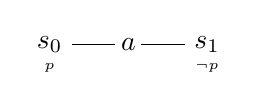
\begin{tikzpicture}[scale = 2.0, every label/.append style = {font=\tiny}]	
			\node[label={[label distance=-0.7cm]:$p$}] (s0) at (0,0) {$s_0$};
			\node[label={[label distance=-0.7cm]:$\neg p$}] (s1) at (1,0) {$s_1$};
		
			\path[every node/.append style={font=\fontsize{10}{0}, fill=white, inner sep=2pt}] 
				(s0) edge node {$a$} (s1);
		\end{tikzpicture}
	} %End scaling
	\break \textit{Note that since we are working with S5 models, all nodes (states) also have reflexive edges to themselves, even if they are not explicitly drawn in these figures}
\end{figure}

\subsection{Language and semantics}

Continuing with the model shown in Figure \ref{fig:basicEM}, we might want to express certain properties or verify that $p$ is indeed true in $(M,s_0)$, for this we would write $(M,s_0) \models p$, or that $s_0$ in the context of $M$ \textit{satisfies} $p$. More formally, $(M,s_0) \models p$ is true \textit{iff} $s_0 \in V(p)$ where if we go back to Definition \ref{def:model}, we can see that V is a valuation function for propositions, meaning that it returns the set of states in $M$, where $p$ is true. 

In general however, we might want to build more complex formulas to check against our models than simple propositions, for this we need connectives; and logics that define their semantics.

\begin{definition}[Group Announcement Logic] \hfill
	\label{def:GAL}
 	\begin{align*}
		\varphi ::= p \ | ~\neg\varphi ~|~ (\varphi~\wedge~\psi) ~|~ (\varphi~\vee~\psi) ~|~ \varphi 							\rightarrow \psi ~|~ K_a\varphi ~|~ [\varphi]\psi  ~|~ [G]\varphi
	\end{align*}
	Where $p$ is a proposition such that $p \in P$, $a$ is an agent i.e $a \in A$ and $G$ is a set of agents i.e $G \subseteq A$
\end{definition}

Definition \ref{def:GAL} defines the language of \lang{GAL} or more specifically, the set of legal formulas that can be built in accordance to GAL. It inductively specifies in BNF-notation how each operator in the language can be used to create new formulas. This notation however merely specifies the \textit{syntax} of the language, which ways we are allowed to arrange the symbols. In order to specify what each operator does, we also need semantics, which we will add through the satisfaction relation $\models$.

\begin{definition}[GAL Semantics] \hfill
	\label{def:GALsem}
	\begin{itemize}
		\item[] $\M,s \models p $ iff $ s \in \vals(p)$
		\item[] $\M,s \models \neg\varphi$ iff $ \M,s \not\models \varphi$
		\item[] $\M,s \models \varphi \wedge \psi $ iff $ \M,s \models \varphi $ and $ \M,s \models \psi$
		\item[] $\M,s \models \varphi \vee \psi $ iff $ \M,s \models \varphi $ or $ \M,s \models \psi$
		\item[] $\M,s \models \varphi \rightarrow \psi $ iff $ \M,s \not\models \varphi $ or $ \M,s \models \psi$
		\item[] $\M,s \models K_i\varphi $ iff for every $t$ such that $s\rels_{i}t$, $\M,s \models \varphi$
		\item[] $\M,s \models [\varphi]\psi $ iff $ \M,s \models \varphi $ implies that $ \M|\varphi,s \models \psi$
		\item[] $\M,s \models [G]\varphi $ iff for every set $\{\psi_i: i \in G\} \subseteq $ \lang{el}, $ \M,s \models [\bigwedge_{i\in G}K_i\psi_i]\varphi$ 
	\end{itemize}
\end{definition}

\todo{Mention tautologies and falsehoods, plus valid and satisfiable formulas ect}

Starting with the most basic component of our formulas we have propositions, commonly referred to as atoms or atomic formulas as propositions themselves are also formulas. If we want to check if some pointed model $\M,s \models p$ or satisfies some property $p$, then as we can see in Definition \ref{def:GALsem} we do this by seeing if the state $s$ is an element in the set of states where $p$ is true, more formally if $s \in \vals(p)$. 

For the explanation of our operators we will be using $\varphi$ and $\psi$ to represent arbitrary formulas. Negation, $\neg$ is relatively trivial, with $\neg\varphi$ simply meaning the negation of $\varphi$ and that $\M,s \models \neg\varphi$ if, and only if $\M,s \not\models\varphi$. Conjunction and disjunction, $\wedge$ and $\vee$ are also pretty simple, translating to `and' and `inclusive or', as can be seen from their definitions in Definition \ref{def:GALsem}. Implication, $\rightarrow$ can be somewhat loosely translated to `if $a$, then $b$', except if $a$ doesn't hold, then the implication automatically holds regardless of $b$. More specifically, the only time an implication is false is when $a$ is true and $b$ is false. We will also use $\varphi \leftrightarrow \psi$, to denote biimplications, meaning $(\varphi \rightarrow \psi) \wedge (\psi \rightarrow \varphi)$ throughout this thesis. 

The previous operators are all relatively basic and only express properties regarding the structures they are checked against, the remaining operators in our language are more interesting, as they also express properties regarding the knowledge of the agents in our systems shifting us towards epistemic logic. The $K_i$ operator is the first of these, with $\M ,s \models K_ap$ expressing that in our pointed model agent $a$ knows that the proposition $p$ is true. Verifying that this is the case however is where things get interesting, as the previous operators only express properties regarding single states, their scope is also limited to that single state, whereas the $K_i$ operator also requires us to check all the states that this agent is incapable of distinguishing from the current state. In order to check if $\M,s \models K_a\varphi$, we need to ascertain that all states a is unable to distinguish from s also satisfy $\varphi$. More specifically, that for all states $t\rels_as$, that $\M,t \models\varphi$. This is because if there exists any such state that does not satisfy $\varphi$, then agent $a$ considers it possible that $\varphi$ is not satisfied since they cannot tell if $t$ or $s$ is the actual state they are in.

While the $K_i$ operator lets us reason around the knowledge of our agents, the public announcement operator $[\varphi]\psi$ lets us update it, or at least add to it by informing the agents through a truthful announcement that some formula is true in the `current' state as defined by the pointed model we are checking the announcement in.
In Definition \ref{def:GALsem} we use the notation $\M|\varphi,s$ to denote $\M$ `updated' by $\varphi$, meaning $\M$ minus all states which do not satisfy $\varphi$.

\begin{definition}[Model Updates]
	\label{def:modupdate}
	$\M$ updated by $\varphi$ is defined as the following: $\M|_\varphi = \langle\states',\rels',\vals'\rangle$ where 
	\begin{align*}
			\states' &= \{s| s\in \states\textrm{ and }\M,s \models\varphi\} \\
			\rels_a' &= \rels_a \cap (\states' \times \states')~ \forall a\in A\\
			\vals'(p) &= \vals(p) \cap \states'~ \forall p \in P
	\end{align*}
\end{definition}

Informally, the definition above in Definition \ref{def:modupdate} can be read as filtering out all states in $\M$ which do not satisfy $\varphi$ and then constraining the equivalence relations for each agent and the valuation function to that filtered set of states.

The final and most interesting operator in \lang{GAL} is $[G]\varphi$, or the group announcement operator, where $G$ is some coalition of agents such that $G \subseteq \ags$. $\M,s \models [G]\varphi$ expresses that there is no way for the group $G$ to announce anything that can make $\varphi$ false in $\M,s$. Note however that the formulas the agents in $[G]$ can announce are constrained to basic epistemic formulas, or to \lang{el} as defined in Definition \ref{def:langel} in order to avoid making our definition of group announcements circular. \todo{Reword sentence} The syntax of $\{\psi_i: i\in G\}[\bigwedge_{i\in G}K_i\psi_i]\varphi$ intuitively means `the conjunction of all formulas $K_i\psi_i$ such that each agent $i$ knows their formula $\psi_i$ and that after this conjunction is announced, $\varphi$ is true'. As the definition in Definition \ref{def:GALsem} specifies that this has to hold for \textit{every} set of $\{\psi_i : i\in G\}$ however, it might be easier to think of it as there not existing a set such that $\M,s \not\models [\bigwedge_{i\in G}K_i\psi_i]\varphi$ or that $G$ does \textit{not} have the ability to prevent $\varphi$ from coming true.

\begin{definition}[Language of epistemic logic \lang{el}] \hfill
	\label{def:langel}
	\begin{itemize}
		\item[] $\M,s \models p $ iff $ s \in \vals(p)$
		\item[] $\M,s \models \neg\varphi$ iff $ \M,s \not\models \varphi$
		\item[] $\M,s \models \varphi \wedge \psi $ iff $ \M,s \models \varphi $ and $ \M,s \models \psi$
		\item[] $\M,s \models \varphi \vee \psi $ iff $ \M,s \models \varphi $ or $ \M,s \models \psi$
		\item[] $\M,s \models \varphi \rightarrow \psi $ iff $ \M,s \not\models \varphi $ or $ \M,s \models \psi$
		\item[] $\M,s \models K_i\varphi $ iff for every $t$ such that $s\rels_{i}t$, $\M,s \models \varphi$
	\end{itemize}
	Where all operators have their semantics defined as in Definition \ref{def:GALsem}
\end{definition}

We will also be using the duality of the two announcement operators, $\langle\varphi\rangle\psi$ and $\langle G\rangle\varphi$ which are defined as follows in Definition \ref{def:dual}.

\begin{definition}[Dual announcement operators] \hfill
	\label{def:dual}
	\begin{align*}
		\M,s &\models \dia{\varphi}\psi\textrm{ iff }\M,s \models \varphi\textrm{ and }\M|_\varphi,s \models \psi \\
		\M,s &\models \dia{G}\varphi \textrm{ iff there exists a set }\{\psi_i:i\in G\} \subseteq \textrm{\lang{el} such that: }\\
			   &\M,s \models \dia{\bigwedge_{i\in G}K_i\psi_i}\varphi
	\end{align*}

\end{definition}

The difference between $[\varphi]\psi$ and $\dia{\varphi}\psi$ is that the box notation `implies' that $\psi$ is true in the updated model, \todo{reword sentence} while the diamond notation requires both that $\M,s\models \varphi$ and $M|_\varphi \models \psi$ For group announcements, the box notation expresses that something has to hold after any possible set of announcements the coalition can make, while the dual $\dia{G}$ expresses that there exists at least one set of announcements for the agents in $G$ such that after their announcements $\varphi$ is true. An interesting observation to make is that like in modal logics we have the same relation between $[\psi]\varphi$ and $\dia{\psi}\varphi$ as $\square\varphi$ and $\lozenge\varphi$, namely that $[\psi]\varphi \leftrightarrow \neg\dia{\psi}\neg\varphi$

When we are discussing announcement operators we are usually also interested in the knowledge of the agents in our system, as such it is useful to be able to refer to the set of states an agent considers indistinguishable from the given state. For this we will be using the notion of equivalence classes, defined as the following:

\begin{definition}[Equivalence classes]
	\label{def:eqclass}
	Given a state $s$ and some agent $a$, a's equivalence class for $s$ is denoted by $\eqc{s}_a$ where
	\begin{itemize}
		\item[] $\eqc{s}_a = \{t~|~s\rels_a t\}$
	\end{itemize}
\end{definition}

Somewhat related to equivalence classes, we will also be using the concept of formula extensions, referring to the set of states a formula is satisfied in, denoted by $||\varphi||$, but also to refer to a set of formulas with the same extension, i.e are satisfied in the same states.

\begin{definition}[Formula extensions]
	\label{def:ext}
	For some formula $\varphi$ and some model $\M$, the extension of $\varphi$ in $\M$ is denoted as $\ext{\varphi}_\M$ where 
	\begin{itemize}
		\item[] $\ext{\varphi}_\M = \{s\in S ~|~\M,s\models\varphi\}$
	\end{itemize}
\end{definition}

\subsection{Bisimulation and bisimilarity}

\question{Hvordan best skille mellom bisimilære tilstander og modeller}

Sometimes we may want to express that two models are `the same', i.e. they satisfy exactly the same set of formulas, despite possibly being structurally different. For this, we have the notion of bisimilarity, denoted by $M \leftrightarroweq M'$. As the concept of bisimilarity is quite central to our exploration of the semantics of the group announcement operator, we introduce the definition of bisimilarity as follows in Definition \ref{def:bisim}

\begin{definition}[Bisimulation]\label{def:bisim}
	Given two models \model{} and \model{'}, a non-empty relation $\bisim\subseteq \states x \states '$  is a bisimulation between $M$ and $M'$ iff for all $s \in \states$ with $(s,s') \in \bisim\mathfrak{:}$
	\begin{description}
		\item[atoms] for all $p \in \props$: $s\in\vals(p)$ iff $s'\in\vals '(p)$;
		\item[forth]  for all $a \in \ags$ and all $t \in \states$: if $s\rels_a t$, then there exists a $t'\in\states '$ such that $s'\rels'_a t'$ and $(t,t')\in\bisim\mathfrak{;}$
		\item[back] for all $a \in \ags$ and all $t' \in \states'$: if $s'\rels'_a t'$, then there exists a $t\in\states $ such that $s\rels_a t$ and $(t',t)\in\bisim\mathfrak{;}$
	\end{description}
\end{definition} 

\begin{figure}[h]
	\label{fig:bisimmods}
	\caption{Two bisimilar, but structurally different models}
	\centering
	\scalebox{1.8}{
		\begin{tikzpicture}[scale = 1.0, every label/.append style = {font=\tiny}]	
			\node[label={[label distance=-0.7cm]:$p$}] (s0) at (0,0.5) {$s_0$};
			\node[label={[label distance=-0.7cm]:$\neg p$}] (s1) at (2,0.5) {$s_1$};
		
			\node[label={[label distance=-0.7cm]:$p$}] (s2) at (4,0) {$s_2$};
			\node[label={[label distance=-0.7cm]:$\neg p$}] (s3) at (3,1) {$s_3$};
			\node[label={[label distance=-0.7cm]:$\neg p$}] (s4) at (5,1) {$s_4$};
		
			\path[every node/.append style={font=\fontsize{10}{0}, fill=white, inner sep=2pt}] 
				(s0) edge node {$a,b$} (s1);
				
			\path[every node/.append style={font=\fontsize{10}{0}, fill=white, inner sep=2pt}] 
				(s2) edge node {$a$} (s3) ++
				(s2) edge node {$b$} (s4);				
		\end{tikzpicture}
	} %End scaling
\end{figure}

Building on the concept of bisimilar states, the bisimulation contraction of a model $\M$ is the smallest bisimilar structure to $\M$, obtained by merging each set of bisimilar states in $\M$ into a single state. 

\todo{Update description of algorithms relating to bisimulation contracting after finishing this clusterfuck}
\begin{definition}[Bisimulation contracted models]
	\label{def:bisimContract}
	Given a model $\M$, one of it's smallest bisimilar structures $\M'$ is 
\end{definition}

The reason why this concept is interesting is that since these bisimulation contracted models do not contain any bisimilar states, this means that per the definition of bisimilarity, there has to exist some set of formulas that uniquely identify each state in our model by being satisfied only in that specific state of our model. We will refer to these as labeling formulas.

\begin{definition}[Labeling formulas]
	\label{def:label}
	Given a bisimulation contracted model $\M$, there exists at least one formula $\varphi_s$ for every $s\in\states$ such that $\M,t \models \varphi_s$ iff $s = t$. More precisely in terms of formula extensions: 
	\centering
	$\forall s\in\states,~\exists\varphi_s$ such that $\ext{\varphi_s} = \{s\}$.
\end{definition}

Additionally, we will also be referring to the set of labeling formulas formulas for a given bisimulation contracted model $\M$ as $\labels{\M}$

\begin{definition}[Set of labeling formulas]
	\label{def:labelSet}
	Given a bisimulation contracted model $\M$, the set of formulas uniquely identifying each state in the model, $\labels{\M}$ is defined as $\labels{\M} = \{\varphi_s | s \in \states\}$
\end{definition}

 \newpage
\section{Group Announcement Logic}\label{sec:theory}

In this section we will introduce and discuss the various concepts and features of epistemic logic, starting by formally defining and explaining the most central concepts we will be working with. We will then present the language of Group Announcement Logic and aim to give the reader an understanding of the semantics behind it, before we transition into our own theoretical work on exploring its group announcement operator in the next chapter. This will lay the foundations for our implementation of the model checking tool that will be presented in the second half of this thesis.

\subsection{Models}

In our introduction we briefly mentioned the concept of Kripke structures and epistemic models. These models are structures consisting of states, typically representing `possible worlds', and agents which may or may not be able to distinguish them. Which states our agents are incapable of distinguishing is represented by an equivalence relation consisting of pairs of states this agent is unable to tell apart and a function from each agent in our model, to that individual agent's equivalence relation. These models also contain a set of boolean propositions, typically describing properties which may or may not hold in each state, as well as a valuation function, which for each proposition in our model, returns the set of states where the given proposition holds.

Throughout the rest of this thesis, we will refer to these models by the following definition: 

\begin{definition}[Models]\label{def:model}
	Given a group of agents $\ags$, and a set of propositions $\props$, a model $\M$ is a structure \model{}, where
	\begin{itemize}
		\item $\states$ is a set of states
		\item $\rels$ is a function from every agent $a \in \ags$ to $a$'s equivalence relation, denoted $\rels_a$, such that $\rels_a \subseteq \states\times\states$
		\item $\vals(p)\subseteq\states$ is a valuation function that for every proposition $p \in \props$ returns the set of states where $p$ is true
	\end{itemize}
\end{definition}

We will also frequently use $\rels$ as $s\rels_a t$, for some $a\in\ags$ to denote that agent $a$ is unable to distinguish between states $s$ and $t$. When we wish to highlight specific states in a model we will denote this by writing $(\M,s)$ to specify that we are referring to state $s$ in the model $\M$, commonly known as a pointed model. This is the form that we will use when we are discussing the properties of a state $s$ in the context of some model $\M$. 

A simple example of an epistemic model could be to imagine someone that doesn't know whether or not it is raining outside. If we focus solely on whether or not it is in fact raining outside, we can denote this proposition as $p$, where $p = $``It is raining outside". Since this agent, $a$ does not know whether it is raining, this means that in their mind there must exist at least two possible worlds, or states; one where $p$ is true, and one where $p$ is false which they are unable to distinguish. If we label these states as $s_0$ and $s_1$, we end up with the model shown in Figure \ref{fig:basicEM}, where we use $\neg p$ to signify that $p$ is not true in $(\M,s_1)$

\begin{figure}[h]
	\centering
	\scalebox{1.9}{
		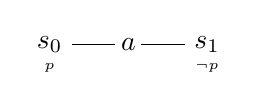
\begin{tikzpicture}[scale = 2.0, every label/.append style = {font=\tiny}]	
			\node[label={[label distance=-0.7cm]:$p$}] (s0) at (0,0) {$s_0$};
			\node[label={[label distance=-0.7cm]:$\neg p$}] (s1) at (1,0) {$s_1$};
		
			\path[every node/.append style={font=\fontsize{10}{0}, fill=white, inner sep=2pt}] 
				(s0) edge node {$a$} (s1);
		\end{tikzpicture}
	} %End scaling
	\caption{A basic model with two states}
	\label{fig:basicEM}
\end{figure}

\textit{Note that since we are working with S5 models, all nodes (states) also have reflexive edges to themselves, even if they are not explicitly drawn in these figures}

\subsection{Language and semantics}

Continuing with the model shown in Figure \ref{fig:basicEM}, we might want to express certain properties such as $p$ being true in $(\M,s_0)$, for this we would write $(\M,s_0) \models p$, or that $\M$ \textit{satisfies} $p$ at $s_0$. More formally, $(\M,s_0) \models p$ holds \textit{iff} $s_0 \in V(p)$ where if we go back to Definition \ref{def:model}, we can see that $V$ is a valuation function for propositions, meaning that it returns the set of states in $\M$, where $p$ holds. 

In general however, we want to build more complex formulas to check against our models than simple propositions, and for this we need connectives; and logics that define their semantics.

\begin{definition}[The language \lang{GAL}] \hfill
	\label{def:GAL}
 	\begin{align*}
		\varphi ::= p \ | ~\neg\varphi ~|~ (\varphi~\wedge~\psi) ~|~ (\varphi~\vee~\psi) ~|~ \varphi 							
		\rightarrow \psi ~|~ K_a\varphi ~|~ [\varphi]\psi  ~|~ [G]\varphi
	\end{align*}
	where $p$ is a proposition such that $p \in P$, $a$ is an agent (i.e. $a \in A$) and $G$ is a set of agents such that $G \subseteq A$.
\end{definition}

Definition \ref{def:GAL} defines the language of \lang{GAL}. It inductively specifies in BNF-notation how each operator in the language can be used to create new formulas. This notation however merely specifies the \textit{syntax} of the language; which ways we are allowed to arrange the symbols. In order to specify what each operator does, we also need semantics, which we will add through the satisfaction relation, $\models$. When some pointed model $(\M,s)$ is not in the satisfaction relation with some formula $\varphi$ (i.e, $\varphi$ does not hold in $(\M,s)$), we write $(+M,s)\not\models\varphi$.

\begin{definition}[GAL Semantics] \hfill
	\label{def:GALsem}
	\begin{itemize}
		\item[] $\M,s \models p $ iff $ s \in \vals(p)$
		\item[] $\M,s \models \neg\varphi$ iff $ \M,s \not\models \varphi$
		\item[] $\M,s \models \varphi \wedge \psi $ iff $ \M,s \models \varphi $ and $ \M,s \models \psi$
		\item[] $\M,s \models \varphi \vee \psi $ iff $ \M,s \models \varphi $ or $ \M,s \models \psi$
		\item[] $\M,s \models \varphi \rightarrow \psi $ iff $ \M,s \not\models \varphi $ or $ \M,s \models \psi$
		\item[] $\M,s \models K_i\varphi $ iff for every $t$ such that $s\rels_{i}t$, $\M,s \models \varphi$
		\item[] $\M,s \models [\varphi]\psi $ iff $ \M,s \models \varphi $ implies that $ \M|\varphi,s \models \psi$
		\item[] $\M,s \models [G]\varphi $ iff for every set $\{\psi_i: i \in G\} \subseteq $ \lang{el}, $ \M,s \models [\bigwedge_{i\in G}K_i\psi_i]\varphi$ 
	\end{itemize}
\end{definition}

Starting with the most basic component of our formulas we have propositions, commonly referred to as atoms or atomic formulas as propositions themselves are also formulas. If we want to check if our pointed model $(\M,s)$ satisfies a property $p$ (denoted by $\M,s\models p$), then as we can see in Definition \ref{def:GALsem} we do this by checking whether the state $s$ is an element in the set of states where $p$ is true, more formally if $s \in \vals(p)$. We denote the fact that the pointed model $(\M,s)$ does not satisfy formula $\varphi$ by $\M,s \not\models\varphi$.

For the explanation of our operators we will be using $\varphi$ and $\psi$ to represent arbitrary formulas. Negation $\neg$, is relatively trivial, with $\neg\varphi$ simply meaning the negation of $\varphi$ and that $\M,s \models \neg\varphi$ if, and only if $\M,s \not\models\varphi$. Conjunction and disjunction $\wedge$ and $\vee$, are also pretty simple, translating to `and' and `(inclusive) or', as can be seen from Definition \ref{def:GALsem}. Implication, $\rightarrow$, can be somewhat loosely translated to `if $a$, then $b$', except if $a$ doesn't hold, then the implication automatically holds regardless of the valuation of $b$. More specifically, the only time an implication is false is when $a$ is true and $b$ is false. We will also use $\varphi \leftrightarrow \psi$, to denote biimplications, meaning $(\varphi \rightarrow \psi) \wedge (\psi \rightarrow \varphi)$ throughout this thesis. 

The previous operators are all relatively basic and only express boolean properties regarding the structures they are checked against, the remaining operators in our language are more interesting, as they also express properties regarding the knowledge of the agents in our systems, shifting us towards epistemic logic. The $K_i$ operator is the first of these, with $\M,s \models K_ap$ expressing that in our pointed model, agent $a$ knows that the proposition $p$ is true. Verifying that this is the case however is where things get interesting, as the previous operators only express properties of the current state, their scope is also limited to that current state, whereas the $K_i$ operator potentially requires us to check every state that this agent is incapable of distinguishing from our current state. In order to check if $(\M,s) \models K_a\varphi$, we need to ascertain that all states a is unable to distinguish from s also satisfy $\varphi$. More specifically, that for all states $t$ such that $t\rels_as$, that $\M,t \models\varphi$. This is because if there exists any such state that does not satisfy $\varphi$, then agent $a$ considers it possible that $\varphi$ is not satisfied since they cannot tell if $t$ or $s$ is the actual state they are in. Hence, the agent is not certain whether $\varphi$ holds.

While the $K_i$ operator lets us reason about the knowledge of our agents, the public announcement operator $[\varphi]\psi$ lets us update it, or at least add to it by informing the agents through a truthful announcement that some formula is true in the current state as defined by the pointed model we are checking the announcement in.
In Definition \ref{def:GALsem} we use the notation $\M|\varphi,s$ to denote $\M$ `updated' by $\varphi$, meaning $\M$ without all states that do not satisfy $\varphi$.

\begin{definition}[Model Updates]
	\label{def:modupdate}
	$\M = \langle\states,\rels,\vals\rangle$ updated by $\varphi$ is defined as the following: $\M|_\varphi = \langle\states',\rels',\vals'\rangle$ where 
	\begin{align*}
			\states' &= \{s| s\in \states\textrm{ and }\M,s \models\varphi\} \\
			\rels_a' &= ~\rels_a \cap (\states' \times \states')~ for ~ all ~ a\in A\\
			\vals'(p) &= \vals(p) \cap \states'~ for ~ all ~ p \in P
	\end{align*}
\end{definition}

Informally, Definition \ref{def:modupdate} can be read as filtering out all states in $\M$ which do not satisfy $\varphi$ and then constraining the equivalence relations for each agent as well as the valuation function to that filtered set of states.

The final and most interesting operator in \lang{GAL} is the group announcement operator, denoted $[G]\varphi$. In $[G]\varphi$, $G$ is some coalition of agents such that $G \subseteq \ags$. $\M,s \models [G]\varphi$ expresses that there is no way for the group $G$ to announce anything that can make $\varphi$ false in $\M,s$. Note however that the formulas the agents in $[G]$ can announce are constrained to basic epistemic formulas, or to \lang{el} as defined in Definition \ref{def:langel} in order to avoid making the definition of group announcements circular. The definition of satisfaction of the group announcement connective reduces to a quantified public announcement (note that this is a different connective with only superficial similarity). It is defined as the statement that the conjuntion of all sets of formulas $\{\varphi_i:i\in G\}$ may be announced without making $\varphi$ false in the current state. More intuitively, that $G$ is unable to avoid $\varphi$ coming about.

The syntax of $\{\psi_i: i\in G\}[\bigwedge_{i\in G}K_i\psi_i]\varphi$ intuitively means `the conjunction of all formulas $K_i\psi_i$ such that each agent $i$ knows their formula $\psi_i$ and that after this conjunction is announced, $\varphi$ is true'. As Definition \ref{def:GALsem} specifies that this has to hold for \textit{every} set of $\{\psi_i : i\in G\}$ however, it might be easier to think of it as there not existing a set such that $\M,s \not\models [\bigwedge_{i\in G}K_i\psi_i]\varphi$ or that $G$ is unable to prevent $\varphi$ from coming true.

\begin{definition}[Semantics of epistemic logic \lang{el}] \hfill
	\label{def:langel}
	\begin{itemize}
		\item[] $\M,s \models p $ iff $ s \in \vals(p)$
		\item[] $\M,s \models \neg\varphi$ iff $ \M,s \not\models \varphi$
		\item[] $\M,s \models \varphi \wedge \psi $ iff $ \M,s \models \varphi $ and $ \M,s \models \psi$
		\item[] $\M,s \models \varphi \vee \psi $ iff $ \M,s \models \varphi $ or $ \M,s \models \psi$
		\item[] $\M,s \models \varphi \rightarrow \psi $ iff $ \M,s \not\models \varphi $ or $ \M,s \models \psi$
		\item[] $\M,s \models K_i\varphi $ iff for every $t$ such that $s\rels_{i}t$, $\M,s \models \varphi$
	\end{itemize}
	where all operators have their semantics defined as in Definition \ref{def:GALsem}.
\end{definition}

We will also be using the duality of the two announcement operators, $\langle\varphi\rangle\psi$ and $\langle G\rangle\varphi$ which are defined as follows in Definition \ref{def:dual}.

\begin{definition}[Dual announcement operators] \hfill
	\label{def:dual}
	\begin{align*}
		\M,s &\models \dia{\varphi}\psi\textrm{ iff }\M,s \models \varphi\textrm{ and }\M|_\varphi,s \models \psi \\
		\M,s &\models \dia{G}\varphi \textrm{ iff there exists a set }\{\psi_i:i\in G\} \subseteq \textrm{\lang{el} such that: }\\
			   &\M,s \models \dia{\bigwedge_{i\in G}K_i\psi_i}\varphi
	\end{align*}

\end{definition}

The difference between $[\varphi]\psi$ and $\dia{\varphi}\psi$ is that the box notation `implies' that $\psi$ is true in the updated model, while the diamond notation requires both that $\M,s\models \varphi$ and $M|_\varphi \models \psi$. For group announcements, the box notation expresses that something has to hold after any possible set of announcements the coalition can make, while the dual $\dia{G}$ expresses that there exists at least one set of announcements for the agents in $G$ such that after their announcements, $\varphi$ is true. An interesting observation to make is that like in modal logics we have the same relation between $[\psi]\varphi$ and $\dia{\psi}\varphi$ as $\square\varphi$ and $\lozenge\varphi$, namely that $[\psi]\varphi \leftrightarrow \neg\dia{\psi}\neg\varphi$ and $[G]\varphi \leftrightarrow \neg\langle G\rangle\neg\varphi$.

When we are discussing announcement operators we are usually also interested in the knowledge of the agents in our system, as such it is useful to be able to refer to the set of states an agent considers indistinguishable from the given state. For this we will be using the notion of equivalence classes, defined as the following.

\begin{definition}[Equivalence classes]
	\label{def:eqclass}
	Given a state $s$ and some agent $a$, a's equivalence class for $s$ is denoted by $\eqc{s}_a$ where
	\begin{itemize}
		\item[] $\eqc{s}_a = \{t~|~s\rels_a t\}$
	\end{itemize}
\end{definition}

Somewhat related to equivalence classes, we will also be using the concept of formula extensions, referring to the set of states a formula is satisfied in, denoted by $||\varphi||$, but also to refer to a set of formulas with the same extension, i.e. are satisfied in the same states.

\begin{definition}[Formula extensions]
	\label{def:ext}
	For any formula $\varphi$ and any model $\M$, the extension of $\varphi$ in $\M$ is denoted $\ext{\varphi}_\M$ and defined as
	\begin{itemize}
		\item[] $\ext{\varphi}_\M = \{s\in S ~|~\M,s\models\varphi\}$
	\end{itemize}
\end{definition}

 Note that as $\eqc{s}_a$ contains all states $a$ is unable to distinguish from $s$, for $a$ to know any formula $\varphi$, this means that $a$'s equivalence class for $s$ has to be a subset of $\varphi$'s extension, as otherwise $a$ would consider it possible that $\varphi$ does not hold. Even stronger, this idea holds both ways, and we get $M,s\models K_a\varphi \Leftrightarrow \eqc{s}_a \subseteq \ext{\varphi}$.

\subsection{Bisimulation}

Sometimes we may want to express that two models are `the same', i.e. they satisfy exactly the same set of formulas, despite possibly being structurally different. For this, we have the concept of bisimilarity, denoted by $\M \leftrightarroweq \M'$. Briefly explained, two models $\M$ and $\M'$ are bisimilar iff for any formula $\varphi$ it holds that $\M,s\models\varphi$ iff there also exists some $s'$ such that $\M',s'\models\varphi$, regardless of $\M$ and $\M'$'s structures. 
%$(\M,s) \leftrightarroweq (\M',s') \Rightarrow \M,s\models\varphi \Leftrightarrow \M',s'\models\varphi$

As bisimilarity will be central to our exploration of the semantics of the group announcement operator in the next chapter, we introduce the definition of bisimilarity as follows in Definition \ref{def:bisim}

\begin{definition}[Bisimulation]\label{def:bisim}
	Given two models \model{} and \model{'}, a non-empty relation $\bisim\subseteq \states \times \states '$  is a bisimulation between $\M$ and $\M'$ iff for all $s \in \states$ with $(s,s') \in \bisim\mathfrak{:}$
	\begin{description}
		\item[atoms] for all $p \in \props$: $s\in\vals(p)$ iff $s'\in\vals '(p)$;
		\item[forth]  for all $a \in \ags$ and all $t \in \states$: if $s\rels_a t$, then there exists a $t'\in\states '$ such that $s'\rels'_a t'$ and $(t,t')\in\bisim\mathfrak{;}$
		\item[back] for all $a \in \ags$ and all $t' \in \states'$: if $s'\rels'_a t'$, then there exists a $t\in\states $ such that $s\rels_a t$ and $(t',t)\in\bisim\mathfrak{;}$
	\end{description}
\end{definition} 

\begin{figure}[h]
	\centering
	\scalebox{1.8}{
		\begin{tikzpicture}[scale = 1.0, every label/.append style = {font=\tiny}]	
			\node[label={[label distance=-0.7cm]:$p$}] (s0) at (0,1) {$s_0$};
			\node[label={[label distance=-0.7cm]:$\neg p$}] (s1) at (2,1) {$s_1$};
		
			\node[label={[label distance=-0.7cm]:$p$}] (s2) at (4,0) {$s_2$};
			\node[label={[label distance=-0.7cm]:$\neg p$}] (s3) at (3,1) {$s_3$};
			\node[label={[label distance=-0.7cm]:$\neg p$}] (s4) at (5,1) {$s_4$};
			\node[label={[label distance=-0.7cm]:$p$}] (s5) at (4,2) {$s_5$};
		
			\path[every node/.append style={font=\fontsize{10}{0}, fill=white, inner sep=2pt}] 
				(s0) edge node {$a,b$} (s1);
				
			\path[every node/.append style={font=\fontsize{10}{0}, fill=white, inner sep=2pt}] 
				(s2) edge node {$a$} (s3) ++
				(s2) edge node {$b$} (s4) ++
				(s4) edge node {$a$} (s5) ++
				(s3) edge node {$b$} (s5);				
		\end{tikzpicture}
	} %End scaling
	\caption{Two bisimilar, but structurally different models.}
	\label{fig:bisimmods}
\end{figure}

Building on the concept of bisimilar states, the bisimulation contraction of a model $\M$ is the smallest bisimilar structure to $\M$, obtained by merging each set of bisimilar states in $\M$ into a single state. 

\begin{definition}[Bisimulation contracted models]
	\label{def:bisimContract}
	A model $\M$ is said to be bisimulation contracted iff there is no model $\M'$ which has fewer states and is bisimilar to $\M$. A bisimulation contraction of a model $\M$, is any minimal model $\M'$, bisimilar to $\M$.
\end{definition}

The reason why this concept is interesting is that since these bisimulation contracted models do not contain any bisimilar states, per the definition of bisimilarity, there has to exist some set of formulas that uniquely identify each state in our model by being satisfied only in that specific state of our model. We will refer to a choice of these as labeling formulas.

\begin{definition}[Labeling formulas]
	\label{def:label}
	Given a bisimulation contracted model $\M$, there exists at least one formula $\varphi_s$ for every $s\in\states$ such that $\M,t \models \varphi_s$ iff $s = t$. More precisely in terms of formula extensions: 
	\centering
	$\forall s\in\states,~\exists\varphi_s$ such that $\ext{\varphi_s} = \{s\}$.
\end{definition}

An important property of these labeling formulas is that the result of publicly announcing a labeling formula will remove all states from our model, except the state this formula uniquely labels. As such, we can reduce our model to any submodel possible, by combining these labeling formulas with disjunctions and announcing the resulting formula. We will additionally be referring to the set of such labeling formulas for a given bisimulation contracted model $\M$ as $\labels{\M}$, defined in Definition \ref{def:labelSet}.

\begin{definition}[Set of labeling formulas]
	\label{def:labelSet}
	Given a bisimulation contracted model $\M$, the set of formulas uniquely identifying each state in the model is defined as $\labels{\M} = \{\varphi_s | s \in \states\}$
\end{definition}


 \newpage
\section{Model checking Group Announcement Logic}\label{sec:algorithms}
%Describe process of translating logical definitions into pseudocode here, then describe model checker in next chapter

In this section we will describe the process of translating the definitions from the previous chapter into algorithms that will be used in our model checker. 

%\todo{Finskrive alt det her, muligens stykke opp og fordele ut etterhvert som det blir relevant}\\
%Before continuing into the translation of defintions into pseudocode, we want to highlight some key differences between the logical definitions of our models and the data structures used in our application. While models themselves are relatively similar, having a set of states and a set of agents, the equivalence relations for each agent and the valuation function for assessing which propositions are true in which states are somewhat different. Our model-structure in the application instead uses a set of edges, pairs of indistinguishable states and which agents consider them so. Secondly it also flips the valuation function in the sense that while the logical definitions define a function which goes from a proposition to the set of states said proposition holds in, our model checker instead goes from a state and returns the set of propositions that hold in that given state.\\

Going back to our revised semantics behind the group announcement operators in Definition \ref{def:GALsemV2} we can see that once we can determine how to enumerate the set of announceable extensions $\anns{G}$, implementing the semantics behind the group announcement operator is fairly straightforward. However, as our definition of $\anns{G}$ uses the concept of bisimulation contracted models, we will first need to cover how we can check whether states are bisimilar and then apply that check to models as a whole in order to reduce them to their smallest bisimilar structures. 

%the definitions of bisimilar states and bisimulation contraction from  and Definition ??? \todo{Actually write definition of bisimulation contraction and refer to it here}. Starting with bisimilarity in general, we will be using the following algorithm for our implementation of bisimilarity checks.
% Discuss basic components of models, states, edges later?
% Skip over algorithms for basic operators

% Repeat why we need bisimilarity check

\subsection{Enumeration of announcements in single agent cases}

Recall the definition of the semantics behind $\M,s \models \dia{G}\varphi$ in Definition \ref{def:dual}, an informal way of explaining it would be that there exists at least one set of formulas the coalition can announce such that $\varphi$ is true after their announcements. 

Using our definitions of labeling formulas and formula extensions in Definition \ref{def:ext} and \ref{def:label} to look at what kinds of formulas any given agent can announce, we note that the goal is to convey information to the other agents in the system. Therefore we do not need to look at the formulas themselves, but only at what consequence announcing them would have and whether or not the agent is able to announce them. For this reason we will be using the concept of formula extensions from Definition \ref{def:ext} instead of concrete formulas as announcing any given formula will eliminate all states not in that formula's extension from the updated model as defined by the semantics of model updates.

\begin{figure}[h]
	\centering
	\scalebox{1.8}{
		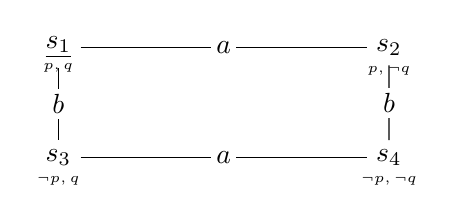
\begin{tikzpicture}[scale = 1.4, every label/.append style = {font=\tiny}]	
				\node[label={[label distance=-0.7cm]:$p,q$}] (s1) at (0,1) {$\underline{s_1}$};
				\node[label={[label distance=-0.7cm]:$p, \neg q$}] (s2) at (3,1) {$s_2$};
				\node[label={[label distance=-0.7cm]:$\neg p, q$}] (s3) at (0,0) {$s_3$};
				\node[label={[label distance=-0.7cm]:$\neg p, \neg q$}] (s4) at (3,0) {$s_4$};
	
				\path[every node/.append style={font=\fontsize{10}{0}, fill=white, inner sep=2pt}] 
					(s1) edge node {$a$} (s2) ++
					(s3) edge node {$a$} (s4) ++
					(s1) edge node {$b$} (s3) ++
					(s2) edge node {$b$} (s4);								
		\end{tikzpicture}
	} %End scaling
	\caption{A basic bisimulation contracted model.}
	\label{fig:GAexample}
\end{figure}

If we attempt to determine which sets of formulas some agent $i$ can announce in the model in Figure \ref{fig:GAexample} we can see that the set of announceable formula extensions will always be a subset of the power set of states in the model. Or more precisely, the set of announceable formula extensions for some agent $i$ in a given pointed model $\M,s$ is a subset of the power set of states in $\M$, where each set is announceable by $i$ if and only if that set follows the following rules in Definition \ref{def:extRules}.

%subset of the power set of extensions of the set of labeling formulas for the model

\begin{definition}[Rules for eliminating formulas by their extension]\hfill
\label{def:extRules}
	For any formula $\varphi$ and bisimulation contracted pointed model $\M,s$, the formula's extension in $\M$, $\ext{\varphi}_{\M}$, must satisfy the following rules in order for the formula to be announceable by some agent $i$ in coalition $G$:
	\begin{itemize}
		\item $\ext{\varphi}_\M$ must contain the actual state in our pointed model
		\item $\forall s\in\ext{\varphi}_{\M}, \forall t\rels_i s \Rightarrow t\in\ext{\varphi}_{\M}$
	\end{itemize}
\end{definition}

The reasoning behind these two rules is based on the semantics of the group announcement operators in Definition \ref{def:GALsem}, we can see that we are essentially searching for a combination of formulas which when announced, make $\varphi$ false. Because of this, having an agent announce that they know something which is false, or something they do not actually know, will simply make the public announcement trivially true. This means there is no point in checking any announcement containing such a formula, therefore the formula:

\begin{itemize}
	\item[(1)] has to be satisfied in the `actual' state of our pointed model
	\item[(2)] has to be satisfied in every state the agent is incapable of distinguishing from that `actual' state
\end{itemize}

\begin{proposition}
For every extension $\ext{\varphi}_{\M}$ that satisfies the rules in Definition \ref{def:extRules} for some agent, any formula with the same extension can be announced by that agent
\end{proposition}

From our definition of formula extensions in Definition \ref{def:ext}, the extension of a formula is simply the set of states in which this formula is satisfied. Therefore if $\varphi$ and $\psi$ share the same extension in some model $\M$, then $\M\models\varphi \leftrightarrow \psi$. From this we can further infer that $\M\models K_a\varphi \leftrightarrow K_a\psi$ for every $\psi$ with the same extension as $\varphi$


\begin{definition}[The set of announceable extensions]\hfill\\
	\label{def:annexts}
	The set of announceable formula extensions $\anns{}$ for some agent $i$, given a pointed model $\M,s$ is defined 			as the following: \\
	$\anns{i,(\M,s)} \subseteq \wp(\{\ext{\varphi}_{\M} ~|~ \varphi\in\labels{\M}\})$ where $\ext{\varphi}_\M \in 		     
	\anns{i,(\M,s)}$ iff it follows the rules in Definition \ref{def:extRules}.
	Note that since every formula in $\labels{\M}$ is only satisfied in a single state in $\states$ and every state in $\states$ satisfies exactly one formula in $\labels{M}$, $\wp(\{||\varphi||_\M ~|~ \varphi \in \labels{\M}\})$ can be simplified to $\wp(\states)$.
\end{definition}

For a more practical explanation we will apply these rules to the model in Figure \ref{fig:GAexample} for agent $a$. Using $s_1$, denoted $1$ in the next example, as the actual state of our pointed model, we start by generating the power set of states in our model and get the following:

\begin{align*}
	\wp(\states) = \{\emptyset,\{1\},\{2\},\{3\},\{4\},\{1,2\},...,\{1,2,3\},...\{1,2,3,4\}\}
\end{align*}
After applying rule (1) from Definition \ref{def:extRules}	to filter out all formula extensions not containing the actual state of our pointed model we get:
\begin{align*}
	\{\{1\},\{1,2\},\{1,3\},\{1,4\},\{1,2,3\},\{1,2,4\},\{1,3,4\},\{1,2,3,4\}\}
\end{align*}
Applying rule (2) to remove all extensions relating to formulas that $a$ does not know leaves us with:
\begin{align*}
	\{\{1,2\},\{1,2,3,4\}\}
\end{align*}

In other words, given the model in Figure \ref{fig:GAexample} agent $a$ is able to announce any given formula $\varphi$ iff $\ext{\varphi}_{\M,1} \in \{\{1,2\},\{1,2,3,4\}\}$. Therefore, $\anns{a,(\M,1)} = \{\{1,2\},\{1,2,3,4\}\}$.

An interesting thing to note here is that we can combine our labeling formulas with disjunctions to create a formula which is satisfied in any subset of the original set of states we want. So for example, in order to create a formula with the extension of $\{s_1,s_2\}$ all we have to do is put disjunctions between the labeling formulas for $s_1$ and $s_2$ such that $\varphi_{\{s_1,s_2\}} = \varphi_{s_1} \vee \varphi_{s_2}$.

If we then want to apply this to checking whether $\M,s_1 \models \dia{a}K_bp$ where $\M$ is still the model in Figure \ref{fig:GAexample} then we can see that since $\{s_1,s_2\}\in\anns{a,(\M,s_1)}$ there exists a formula extension that $a$ can announce which would eliminate $s_3$ from the model. This would cause $K_bp$ to be satisfied in the updated model and therefore satisfy $\dia{a}K_bp$.

\subsection{Generalizing the single agent case}

Expanding what we have presented so far to encompass coalitions comprised of multiple agents is actually very easy. 
When we are assessing the ability of an agent to announce something which may change the valuation of a formula, we are simply checking whether or not that agent is capable of eliminating certain states in the updated model. In other words, if we wish to assess the ability of a whole coalition, all we need to do is look at which sets of states each agent in the coalition is able to eliminate in unison.

An interesting observation to make is that an agent $i$ is always capable of eliminating any state they can distinguish from the actual state of some pointed model. This means that in order to find out which states a coalition can eliminate, we can simply take the power set of states and limit it to the combinations of states which fit the rules of Definition \ref{def:extRules}, where we slightly tweak rule 2 to the following:

\begin{definition}[The set of extensions announceable by coalitions]
	\label{def:extscoal}
	The set of announceable extensions $\anns{G,(\M,s)}$ for some coalition $G$, given a bisimulation contracted pointed model $\M,s$ is defined as the following: \\
	$\anns{G,(\M,s)} = \{\states' \subseteq \states ~|~ \forall s'\in \states', \neg\exists t\forall i\in G ~ t\rels_i s', t\not\in \states' \textrm{ and } s\in\states'\}$
\end{definition}

A candidate set $\states'\subseteq\states$ not satisfying the condition is clearly not announceable because it contains a state $s$ which no agent in the coalition can distinguish from the excluded state $t$.

\subsection{Proof of suitability}

In this section we will compare our definitions and work so far with the definitions presented by Ågotnes et al. in their paper on GAL. In their paper they describe how to check formulas of the kind $\dia{G}\varphi$ in the following manner:

\begin{definition}[Definition of $\dia{G}\varphi$ by Ågotnes et al.]
	\label{def:GALsemAagotnes}
	$\M,s\models \dia{G}$ iff there is a definable restriction $\M'' = (\states'',\rels'',V')$ of $\M$  such that $\states'' = \cap_{i\in G}C_i$ where  $C_i$  are unions of classes of equivalence for $\rels_i$ and $s\in\states''$ and $\M',s\models\varphi$
\end{definition}

Decomposing their definition we end up with $\states''$ being the intersection of the unions of some subset of each agent's equivalence relation. More specifically, for each agent $i$, we choose which equivalence classes 
should be part of that agent's union of equivalence classes $C_i$ and then check if there exists some combination of values for each $C_i$ such that restricting the set of states to the intersection of these $C_i$s gives us a model which both contains the original state $s$ and satisfies $\varphi$.

Comparing this definition to our definition of the announceable set of extensions for a coalition, we argue that our definition of $\anns{G,(\M,s)}$ defines exactly these intersections of possible combinations of $C_i$s from the definition of Ågotnes et al. If we further decompose their definition, we end up with the two following restrictions:
\begin{align}
	&S'' = \bigcap_{i\in G}C_i \textrm{ where } C_i \subseteq S, \forall s\in C_i, \eqc{s}_i\subseteq C_i \\
	&s \in S''
\end{align}

From this, we argue that our definition of $\anns{G,(\M,s)}$ incorporates the same two restrictions, in turn quantifying the set of all possible restricted sets $\states''$. Decomposing our definition the same way we did Definition \ref{def:GALsemAagotnes}, we end up with $\anns{G,(\M,s)}$ defined as the set of all subsets of $\states$, $S'$ which satisfy the following two restrictions:
\begin{align}
	&\forall s'\in S' \neg\exists t\forall i \in G, t\rels_i s', t\not\in S' \\
	&s\in S'
\end{align}

Expanding on our restriction in $(3)$, we could write it out as `if there exists a state $t$ indistinguishable by all agents from $s$, then either $t\in S'$ or $s\not\in S'$'. A simpler way of phrasing this would be to say that for every state in $S'$, the intersection of its equivalence classes for all agents in the coalition has to be a subset of $S'$. Changing (3) to fit this simpler phrasing gives us
\begin{align}
	\forall s'\in S' \cap_{i\in G}\eqc{s'}_i\subseteq S'
\end{align}

which should further clarify that combining restriction $(4)$ and $(5)$ provides the same set of possible values as $(1)$ and $(2)$. Based on this, we revise the semantics for the group announcement operators into the following:

\begin{definition}[Group announcement operators, revised]
	\label{def:GALsemV2}
	\begin{align*}
		\M,s & \models [G]\varphi \textrm{ iff }  \forall Ext\in\anns{G,(\M,s)} \textrm{ then } \M,s\models [\varphi_{Ext}]\varphi\\
		\M,s & \models \dia{G}\varphi \textrm{ iff } \exists Ext\in\anns{G,(\M,s)} \textrm{ such that } \M,s\models \dia{\varphi_{Ext}}\varphi
	\end{align*}
	where $\varphi_{Ext}$ is a formula of the form $\bigvee_{s\in Ext}\varphi_{s}$
\end{definition}

Our reason for revising these definitions is that the original definitions in \ref{def:GALsem} define satisfaction of $[G]\varphi$ by using a quantifier over an infinite set of formulas making it unfit for our goals of implementing a model checking tool. We will therefore be implementing the revised definition in \ref{def:GALsemV2} instead as the set of announceable extensions is far easier to enumerate than the set of announceable formulas. This is still equivalent to the original definition as we are simply grouping the infinite set of announceable formulas into a finite set of announceable extensions.

\subsection{Algorithm for bisimilarity check}

Using the definition of bisimilarity in Definition \ref{def:bisim} we present our recursive function for checking bisimilarity between states. Given a set of states $States$, a set of agents $Agents$ and two states $s$ and $s'$ such that $s, s' \in States$, the function (recursive bisimulation check) $rbc(s,s',States, Agents)$ determines whether $s$ and $s'$ are bisimilar is defined as Algorithm \ref{alg:rbc}.

\begin{algorithm}
\caption{Recursive Bisimulation Check}
\label{alg:rbc}
\begin{algorithmic}[H]
\Function{$rbc$}{$s,s',States,Agents$}
	\If {$s = s'$}
		\State\Return $true$
	\ElsIf{$props(s) \ \neq \ props(s')$}
		\State\Return $false$
	\ElsIf{States = $\O$}
		\State\Return $true$
	\Else
		\State $States' \gets States \setminus \{s,s'\}$
		\State $forth \gets$ \Call{$knowledgeCheck$}{$s,s',States',Agents$}
		\State $back \gets$ \Call{$knowledgeCheck$}{$s',s,States',Agents$}
		\State \Return $(forth \ and \ back)$
	\EndIf
\EndFunction
\end{algorithmic}
\end{algorithm}

The resulting algorithm is fairly similar to the logical definition, with the $props$ check being equivalent to the $atoms$ clause and the $knowledgeCheck$ function replacing the $forth$ and $back$ clauses. Note that our valuation function is flipped, going from a state to a set of propositions, rather than a proposition to a set of states. The pseudocode for the $knowledgeCheck$ function used to translate $forth$ and $back$ is shown in Algorithm \ref{alg:kc}.

\begin{algorithm}
\caption{Knowledge Check}
\label{alg:kc}
\begin{algorithmic}
\Function{$knowledgeCheck$}{$s,s',States,Agents$}
	\ForAll{$(t, Ags) \ in \ neighbours(s,Agents, States')$}
		\ForAll{$a \ in \ Ags$}
			\State $hasMatching \gets false$
			\ForAll{$(t', Ags') \ in \ neighbours(s', Agents, States')$}
				\If{$a \in Ags'$ and \Call{$rbc$}{$t,t',States',Agents$}}
					\State $hasMatching \gets true$
					\State $\mathbf{break}$
				\EndIf
			\EndFor
			\If{!hasMatching}
				\State\Return $false$
			\EndIf
		\EndFor	
	\EndFor
	\State \Return $true$ 
\EndFunction
\end{algorithmic}
\end{algorithm}

Comparing our algorithm to the original definition of bisimilarity the main point of interest is how it is finite, since for each recursive call to $rbc$ we prevent the two current states from being checked again, meaning that at some point the algorithm is guaranteed to halt. The function $neighbours$ used in the $knowledgeCheck$ function simply returns a set of tuples for each state visible from $s$ and the set of agents it is visible to, limited to states in $States$.

\subsection{Smallest bisimilar structure}

Building on the previous algorithm, the next step is using it to create an algorithm for constraining a model to one of its smallest bisimilar structures, by filtering out all bisimilar states. While we normally would not need to worry about which states are filtered, as we are generating a checking log to visualize the checking process for our users, we wanted to avoid having the `actual' state of our pointed model filtered out. As such, we simply make sure that the actual state lies first in our set of states when calling $bisimContract$ in our application. 

\begin{algorithm}
	\caption{Bisimulation contraction}
	\label{alg:bisimContract}
	\begin{algorithmic}
		\Function{$bisimContract$}{$States, Agents, Edges$}
			\State $bisimMap \gets Map<State, State>$
			\ForAll{$(state) \ in \ States$}
				\ForAll{$(otherState) \ in \ States \setminus (state \ \cup \ keys \  in \ bisimMap) $}
					\If{\Call{$rbc$}{$state, otherState, States, Agents$}}
						\State \Call{$bisimMap.put$} {$otherState, state$}
					\EndIf
				\EndFor
			\EndFor
			\State $CS \gets States \ \setminus \ (keys \ in \ bisimMap)$
			\State $CE \gets \{ e \in Edges ~|~ e.state1 \not\in CS \ and \ e.state2 \not\in CS\}$
			\State $contractedModel \gets (CS, Agents, CE)$
			\State \Return $contractedModel$
		\EndFunction
	\end{algorithmic}
\end{algorithm}

\question{Burde ikke filteret i CE 'flippes'? Altså at $startState(e) \in CS$?}

\subsection{Enumerating the set of announceable extensions}

As we have now laid the groundwork of formulating how we can compute bisimulation contractions of models, we can move on to presenting how we can generate the set of announceable extensions. For this we will be using the definition of announceable extensions presented in Definition \ref{def:extscoal}. While Ågotnes et al.'s definition in \ref{def:GALsemAagotnes} is more compact, our definition more closely resembles its pseudocode translation.

\begin{algorithm}
	\caption{Generating a coalition's set of announceable extensions}
	\label{alg:genAnnExts}
	\begin{algorithmic}
		\Function{$genAnnExts$}{$contractedModel, actState, coalition$}
			\State $states \gets contractedModel.states$
			\State $extensions \gets \wp(states)$
			\ForAll {$extension ~ in ~ extensions$}
				\If {$actState \not\in extension$}
					\State remove $extension$ from $extensions$
				\Else
					\ForAll {$state$ in $extension$}
						\State $eqClass \gets $\Call{$genEqClass$}{$state, states, coalition$}
						\ForAll {$eqstate$ in $eqClass$}
							\If {$eqstate \not\in extension$}
								\State remove $extension$ from $extensions$
								\State $\mathbf{break}$
							\EndIf
						\EndFor
					\EndFor
				\EndIf				
			\EndFor
			\State \Return $extensions$
		\EndFunction
	\end{algorithmic}
\end{algorithm}

As can be seen, the algorithm for generating the set of announceable extensions boils down to generating the power set of states in the model, i.e. the set of all possible extensions, and then filtering it according to the rules in Definition \ref{def:extRules}. The $genEqClass(state, agents)$ function used is mostly identical to the $neighbours$ function used previously, except it returns the list of states that the coalition as a whole considers indistinguishable from the input state. 

Now that we have not only our bisimulation contracted model, but also a way to generate all of the announceable formula extensions for any coalition, describing the algorithm for checking group announcement formulas becomes straightforward. As these extensions are really just stand-ins for some announcement made by the agents as per the original definition in Definition \ref{def:GALsem}, we can also regard them as constraints on our model. Going by our revised definition of the semantics behind the group announcement operator from definition \ref{def:GALsemV2}, all our algorithm needs to do is to check whether all of the constrained models we get from applying these constraints to our bisimulation contracted model satisfy the post condition of the group announcement. As such, we translated the semantics of the group announcement operator into the following checking function, shown in Algorithm \ref{alg:checkGroupAnn}.

%Discuss optimizations in regards to non-epistemic formulas not changing valuation through announcements\\
\begin{algorithm}
	\caption{Check function for group announcement operator}
	\label{alg:checkGroupAnn}
	\begin{algorithmic}	
		\Function{$check_{[G]\varphi}$}{$state, innerForm, model, coalition$}
		\State $contractedModel \gets$ \Call{$bisimContract$}{$model$}
		\State $extensions \gets $\Call{$genAnnExts$}{$contractedModel, state, coalition$}
		\ForAll {$extension$ in $extensions$}
			\State $constMdl \gets$ \Call{$constrainMdlBy$}{$contractedModel, extension$}
			\State $extSatisfiesForm \gets $ \Call{$check$}{$state, innerForm, constMdl, coalition$}
			\If{$!extSatisfiesForm$}
				\State \Return $false$
			\EndIf
		\EndFor
		\State \Return $true$
		\EndFunction
	\end{algorithmic}
\end{algorithm}

Like we previously mentioned we here make sure the set of states passed to $bisimContract$ starts with the actual state we're checking our formula in, in order to simplify the visualization of our checking process. It should also be mentioned that the $check$ function that gets called is implemented as an abstract function overridden by each operator in our system and that Algorithm \ref{alg:checkGroupAnn} only shows the implementation for the group announcement operator. The $constrainMdlBy$ function used here is merely a special case of updating a model through announcing the set of states directly instead of announcing a formula and constraining our model to the set of states that satisfy the given formula. 

\todo{Show algorithms for checking conjunctions, knowledge and public announcements}

Now that we have presented our algorithm for checking group announcements, we will additionally present our checking algorithms for a few of the simpler operators as well. Starting out, we present Algorithm \ref{alg:checkConj} for checking conjunctions. As all of the non-epistemic operators can be checked in similar fashion with only minor tweaks to the algorithm, we will be skipping the rest of them and instead move on to the knowledge operator. 

\begin{algorithm}
	\caption{Check function for the conjunction operator}
	\label{alg:checkConj}
	\begin{algorithmic}
		\Function{$check_{\varphi\wedge\psi}$}{$state, leftForm, rightForm, model$}
		\State $leftSatisfied \gets $ \Call{$check$}{$state, leftForm, model$}
		\If{$leftSatisfied$}
			\State \Return \Call{$check$}{$state, rightForm, model$}
		\Else
			\State \Return $false$
		\EndIf
		\EndFunction
	\end{algorithmic}
\end{algorithm}

Algorithm \ref{alg:checkKnowledge} describes how we check knowledge in our model checker. The $getIndishStates$ function we use here returns the set of states an agent considers indistinguishable from the given state, which is then looped over as we check whether the `inner' formula is satisfied in all these indistinguishable states.

\begin{algorithm}
	\caption{Check function for knowledge operator}
	\label{alg:checkKnowledge}
	\begin{algorithmic}
		\Function{$check_{K}$}{$state, innerForm, agent, model$}
		\State $indistinguishableStates \gets $ \Call{$getIndishStates$} {$state, agent$}
		\ForAll {$indishState$ in $indishtinguishableStates$}
			\If {!\Call {$check$}{$indishState, innerForm, model$}}
				\State \Return $false$
			\EndIf
		\EndFor
		\State \Return $true$
		\EndFunction
	\end{algorithmic}
\end{algorithm}

Finally, we also present Algorithm \ref{alg:checkPubAnn} for checking public announcements, which also serves to highlight a few interesting deviations 
\todo{Skrive ferdig}

\begin{algorithm}
	\caption{Check function for public announcements}
	\label{alg:checkPubAnn}
	\begin{algorithmic}
		\Function{$check_{[\varphi]\psi}$}{$state, announcement, innerForm, model$}
		\State $updStates \gets List <State>$
		\ForAll {$state$ in $model.states$}
			\If {\Call {$check$}{$state, innerForm, model$}}
				\State $updStates.add(state)$
			\EndIf
		\EndFor
		\State $updEdges \gets List <Edge>$
		\ForAll{ $edge$ in $model.edges$}
			\If {$edge.state1 \in updStates$ and $edge.state2 \in updStates$}
				\State $updEdges.add(edge)$
			\EndIf
		\EndFor
		\State $updModel \gets$ \Call {$updateModel$}{$updStates, updEdges, agents$}
		\State \Return \Call {$check$}{$state, innerForm, updModel$}
		\EndFunction
	\end{algorithmic}
\end{algorithm}

\question{Bruke $List<Foo>$ eller $Foo[~]$? Evt hva med $Map<State, State>$?}

Note that we can also check if $state \not\in updStates$ and immediately return true if this is the case. \newpage
%Test formulas for Muddy Children:
%[ma|(mb|mc)][(!KA(ma))&((!KB(mb))&(!KC(mc)))]KB(mb)
%

\section{Model checking}\label{sec:impl}


 \newpage
\section{Implementation}\label{sec:impl}

* Discuss how formulas are interpreted / parsed into tree-structures where each the nodes themselves 'contain' definitions for the semantics behind the logical connective they represent, based on their class.
* Refer back to previously presented algorithms when discussing recursive checking function
* Refer back to background chapter when discussing why the problem is interesting when presenting artifact.
* Model checking often limited to yes / no questions, discuss added value by transcending boolean 

\todo{Mention inspiration from JFLAP and experience with using it as educational tool}
%JFLAP, a tool previously used here at our faculty to teach students how turing machines and finite state automatas work.


In this chapter we will present our own implementation of a model checker for Group Announcement Logic called \cname and describe its inner workings. Our initial goal with \cname was to create an educational tool that could aid students with learning epistemic logic in a more visual manner. Therefore, while most other model checking utilities such as DEMO \cite{JanvanEijck} stick to answering the user's queries with simple yes and no answers, we wanted to go beyond that by showing them not just whether their formulas hold, but also visualize why and provide the user with an easier, visual way of drawing models almost as they would on paper or blackboard. The reasoning behind this was that by allowing the user to manipulate the model through a simple click-and-drag interface and seeing how it can affect the valuation of various formulas they might gain a deeper understanding of the semantics involved.


\subsection{Generating examples}

As our motivation behind creating \cname was to create a learning tool that could help new logicians understand how the semantics of GAL work, being able to generate examples which highlight interesting properties of our models is highly important. As such, MCGAL was designed from the ground up to be able to trace its steps through the model checking process so that it can also display each step of this process in an intuitive manner. The program therefore creates a log entry each time it checks an operator against a specific state in the model, keeping track of sub-formulas and formula depth as it goes through the operators. The reason behind also keeping track of sub-formulas and formula depth in the logs is to create a more easily navigable tree-like structure. This tree-structure facilitates skipping through chunks of the process that might not be particularly interesting to the user, allowing them to for example view each state the tool checks against a particular K-operator, or even skip through each of the possible updated models a coalition can reduce a model to through their announceable extensions, without having to step through the checking of the inner formula every time.

\begin{figure}[H]
	\label{fig:basicGalChecking}
	\caption{Checking a basic group announcement formula in MCGAL}
	\includegraphics[width= \textwidth]{MCGALBasicChecking.png}
\end{figure}

As the tool provides a view of the model, it also updates this view by showing what the model it is currently checking against looks like, by highlighting the state and operator the tool is currently checking as well as graying out any states that have been filtered out by model updates. Examples of such model updates might be constraining the model to one of the formula extensions a coalition can announce, which is what is being displayed in Figure \ref{fig:basicGalChecking}. In this example, we are checking whether the formula $\neg [Bob]\neg KAnn[p]$ holds in state s3 of our model. The formula roughly translates to: 'It is not the case that Bob is unable to make Ann know $p$' or more simply in its dual form: 'Bob is able to make Ann know p'. From the visualization of our model in Figure \ref{fig:basicGalChecking} we can see that since Bob is able to reduce the model to only states where $p$ holds, Ann also trivially knows that $p$ holds in this updated model, satisfying our original formula. In this somewhat trivial example, the tool ended up only having to try announcing a single formula extension before it found an extension that made our original formula true. If we were to check a more complex formula however, it might end up checking tens of different announcements, each generating a different updated model after its announcement which the tool will helpfully visualize, giving the user insight into a coalition's capabilities. Note that the previous example could also have been made easier by rewriting the formula as $\dia{Bob}KAnn[p]$, but unfortunately the tool does not (yet) support diamond operators. 


\begin{figure}[h]
	\label{fig:debugExmpl}
	\caption{Example of using \cname's step-by-step formula checking}
	\includegraphics[width=\textwidth]{DebuggerExample.png}
\end{figure}

%Admittedly UX and design in general is not my strong suit and improving the interface is left as future work
%They would additionally be able to type in a formula and then have the states in their model light up, highlighting which states satisfy the given formula. 

Another key feature of the application is that in addition to simply checking which states in the user's model satisfy their fomula, they can also look more closely at why a formula is or is not satisfied in a given state. In order to help the user with this, the application visualizes the checking process step-by-step, one operator and state at a time, with progress being displayed by updating the color of each operator in the formula according to their current valuation.


Figure \ref{fig:debugExmpl} shows a screenshot of \cname in action, where the user is stepping through the process of checking a specific formula against a state in their model, having the tool visualize whether or not their formula holds. It also shows how the application breaks down epistemic formulas into sub-formulas and display them next to each state they have to be checked in. Additionally, the application also visualizes the current valuation of each operator and proposition in the formula as you step through the checking process, as can be seen from the red and green parts of the formulas being checked, as well as the Val column in the debugger tab. Note that the user can also step forwards or backwards through this process at any time by either clicking the step they want to skip to, or browsing with the arrow keys. 


\subsection{Choice of platform}

\subsection{Language and interpretation}

\subsection{Model checking}


\subsection{Tech choices}

Our model checker was implemented in Kotlin as it is a new and exiting language while also being based on the JVM, providing access to the wast libraries and tools written for Java, including JavaFX and a Java hook for ANTLR which will be discussed in more detail later in this section. Kotlin additionally has a smooth and concise syntax as well as lending itself very well towards writing functional code despite being object oriented through shorthands for lambda expressions, support for proper function types and distinctions between mutable and immutable structures and variables. Among the other benefits of the language is that Kotlin being a relatively fresh and recent language, is that it has been able to draw plenty of inspiration from other  meaning it also has lots of lovely `modern' language features such as type inference, string interpolation and default values for making function arguments optional, meaning you no longer have to write three different constructors as one would in good old Java. While the language is still relatively young, being first unveiled in 2011\cite{KotlinHello}, it is being backed by Jetbrains, who are well known for their suite of plugins and IDEs such as IntelliJ and PyCharm, meaning the language has excellent tooling support despite its age.

As for the choice of graphics library to build the application's user interface in, the choice fell on a Kotlin wrapper for the de facto standard Java GUI library of JavaFX, called TornadoFX\footnote{Library homepage at: \url{https://tornadofx.io}}. While JavaFX is a widely used and mature library with powerful features, we also feel it tends to be somewhat clunky and verbose unless one dumps the layout and positioning of components into specialized XML-files. While this helps clean up classes representing UI-components, we also find it makes dynamic component generation clumsier. Our reasons for wanting to use TornadoFX over plain JavaFX is that TornadoFX, being a Kotlin library is able to have a much cleaner and prettier API by utilizing Kotlin features such as lambda expressions attached to receivers to create composable builder functions which generate your JavaFX component hierarchy in an imperative fashion. Another excellent feature of TornadoFX is its concise shorthands for creating dynamic bindings between UI components and observable sets of data. An example of this would be using the standard bindChildren() function to dynamically create and destroy UI components representing states in the user's epistemic model based on changes to that internal list of objects which represent states in a single line of code, by simply feeding the bindChildren() function a reference to the observable list of states and a transformation function that converts the data structure representing a state, to the corresponding UI component, in our case simply the constructor of this component. If anything, I would say that TornadoFX's greatest feature is how its composable builder functions allows you to circumvent the normally inverse order of declaration and creation of UI components compared to their order in the component hierarchy, which can be seen in Figure \ref{fig:StatFragSnip}. \todo{Find out why Latex is fucking up this reference}

\begin{figure}[h]
	\label{fig:StatFragSnip}
	\caption{Code handling how the UI components representing states are built. Note the conciseness due to implicit contexts.}
	\includegraphics[width=\textwidth]{StateFragmentSnippet.png}
\end{figure}

As for parsing the formulas, I went with ANTLR\footnote{\url{http://www.antlr.org/}} for generating the parsers I needed. ANTLR is a pretty powerful tool for generating parsers and lexers based on easily definable grammatical rules like the ones in Figure \ref{fig:grammar}

\begin{figure}[h]
	\label{fig:grammar}
	\caption{Grammatical rules for parsing formulas in \cname with ANTLR. }
	\includegraphics[width = \textwidth]{GALGrammar.png}
\end{figure}

These grammatical rules are used by ANTLR to generate parser and lexer classes which implement these rules in a manner that allow me to easily translate from raw text and lexical tokens into data structures of my own design which represent the various operators and encapsulate their semantics. One thing to note in Figure \ref{fig:grammar} are the signs used to represent negation, conjunction and disjunction. As the commonly used symbols for these operators do not exist on normal keyboards, the UI would either need extra buttons to facilitate inserting these symbols or use more easily inputable surrogate symbols. I chose the latter, going for the boolean equivalents of using exclamation marks for negations, not, ampersand for conjunctions, and, as well as the vertical bar, or `pipe' character commonly representing the or operator. Note that \cname automatically converts these characters to their `correct' symbols when displaying the input formula however, as can be seen in figure \ref{fig:debugExmpl}. 
Another small concession I had to make in order to differentiate between agents and propositions was to force agent names to be capitalized as I would otherwise have to resort to using different symbols to differentiate between regular public announcements and group announcements. Due to time constraints, the dual diamond announcement operators were not implemented, but both the grammar as well as the formula structures should be easily extendable in order to implement them as future work.

\subsection{Implementation details}

As the focus when making the application was mainly on making the it as easy to use as possible while presenting information in a visual manner that is easy to grasp, we ended up making several deviations from the logical definitions of the various structures that have been discussed throughout the thesis. Here we will discuss some of them as well as why these deviations were useful to us. Additionally we will also describe the inner workings of our tool, the technologies and frameworks it is built on as well as our reasons for choosing these.

A key difference here is how we chose to represent the components of our epistemic models themselves.  In Definition \ref{def:model} we present $\rels$ as a function from each agent to their respective equivalence relation for every state in the model, whereas in \cname we instead chose to represent these equivalence relations as a set of edges represented as objects consisting of pairs of states and sets of agents. The reasons for this ties back into how we wanted to present an interactive view of the models in our application as it felt cleaner represent each edge between states as a concrete objects which we could then bind a UI-component to, than hold onto sets of sets of states for each agent. Since each edge also has a reference to the set of agents it is valid for, it becomes trivial to visualize this information as well.

We also chose to flip the valuation function by letting states hold a reference to the set of propositions they satisfy rather than each proposition being linked to the set of states they are satisfied in. Our reasoning here is much the same as we highlight which propositions are true in which states through bindings to each state's set of propositions, which is far simpler than having to go through the entire set of propositions each time the user updates which propositions a given state satisfies. An example of how this looks can be seen in Figure \ref{fig:basicModelVis}, with both states and the edges between them being just bindings to simple data structures, updating whenever their underlying data does.

\begin{figure}[H]
	\label{fig:basicModelVis}
	\caption{A basic model, visualized in \cname}
	\includegraphics[width= \textwidth]{BasicModel.png}
\end{figure} 

Additionally, we also made each state aware of which edges it is connected to, trivializing the logic behind finding `neighboring' states for a given agent as we simply filter the set of edges our state is connected to based on each edge being valid for said agent and return a list of states these edges lead to.

Continuing our discussion of how we implemented our formula structures in \cname, we use a text parser generated from a small ANTLR grammar file in order to parse formulas entered by the user into a tree-like structure representing their formula. When checking this formula the user then has a choice of whether they simply want to see which states in the model satisfy their formula, or whether they want a more detailed visualization of why their formula is or is not satisfied in a specific state. If the user then opts for the first option and check their formula against the whole model, then the tool will highlight the states as either green or red, depending on whether that state satisfies the input formula. The tool also generates an interactive visual representation of the formula where the user can mouse over each operator to check the sub-formula that operator represents against the model as seen in Figure \ref{fig:labelHover}. The idea behind this being that the user might be interested in quickly seeing which states in their model satisfy the various sub-formulas to help better understand how the original operator works. The way this was implemented was to basically create UI components for each operator in the formula and the sub-formula they represent and then check each sub-formula against the model as the user mouses over them, highlighting which part of the formula they represent.

\begin{figure}[H]
	\label{fig:labelHover}
	\caption{Illustration of interactive formula display}
	\includegraphics[width= \textwidth]{LabelMouseOver.png}
\end{figure}

How step-by-step visualization works is somewhat more involved. A high-level description of how it is implemented is that the `debugger' hooks into the $check$ function of the formula, and logs each step of the checking process. Each log then carries information about what the valuations of each operator was at that point in the process, so that this checking process can be played back and visualized in the form of showing the various operators change color as their valuations become known. One pretty cool feature of this step-by-step visualization is that it allows the user to see which states get filtered out by model updates and even see the checking process play out in each formula extension a given coalition can announce in the case of checking group announcement formulas. There were also plans for separately visualizing the set of announcements a coalition can make as well as showing what the updated models would look like, but unfortunately this had to be scrapped due to time constraints.

\begin{figure}[H]
	\label{fig:formulaImpl}
	\caption{Snippet showing how various operators are implemented}
	\includegraphics[width=\textwidth]{FormulaImpl.png}
\end{figure}

%Features - should explain how each of these are implemented \\\\

%Simple click-and-drag interface for creating models\\
%Reinventing the wheel in terms of click-and-drag\\
%Saving and loading models, as well as importing other models into the current model (Useful for importing commonly used components)\\
%Visualizing which states satisfy a given formula, and being able to mouse over sub-formulas to check them as well\\
%When using the step-by-step visualizer, the user can skip over sub-formulas as the application keeps track of operator depth\\

\todo{Create UML diagram of data structures and how they are connected}

%Models - $M = \{states, agents, edges, props)\}$\\

%States - 'Know about' edges they are connected to, 'know' which propositions they satisfy in order to ditch hassle of valuation function (Instead of $V(p) \rightarrow \{s\}, V(s) \rightarrow \{p\}$)\\

%Edges - Are actual objects rather than part of some equivalence relation, easier to deal with, more direct in terms of knowing what to render and interact with (Also in terms of traversing, knowing which states to interact with without having to go through a bunch of sets, i.e equivalence relations)). 'Know about' which agents they represent and which states they are between\\

%Formulas - \\

%Compare with implementations in DEMO, advantages/disadvantages of wrapping things in objects ect.\\
%We use observable objects with pointers to each other, DEMO simply has arrays of integers, which are more lightweight and potentially easier to manipulate, but much harder to render \\
%Discuss differences with logical definitions\\
%Provide walkthrough of how program checks formulas\\

%Debugger, DebugLabels, attaching itself to checking process of formulas, lots of shady voodoo to link DebugEntries in sidepanel to DebugLabels next to each state in order to update them as the user navigates through entries\\

%Debugger inserts callback into CanvasController to know when the user selects a state\\
%List of checking steps has onChange() callback telling the Debugger to apply the valuation map for that step to all formula labels\\

%Checking: Everything up to knowledge is roughly equivalent to logical definitions, minus flipped valuation function. Knowledge is similar, but instead of having an equivalence relation for each agent, each state is instead connected to other states through a set of edges which hold for a set of agents. If 


%Checking, recursive, 'logger' used to display process step-by-step\\

\subsection{Future work}

\todo{Skrive om å måle pedagogisk verdi, muligens peke ut som fremtidlig masteroppgave}

Having developed what we consider to be a potentially highly useful education tool, the big elephant in the room when discussing future work is actually measuring its educational benefit. As both user testing and educational impact studies go beyond the scope of this thesis, we certainly hope that someone might be willing to take up the torch and prove the value of \cname in such settings. While \cname is fully functional and usable as an educational aid in its current state, there are also a fair few features that we simply did not have time to implement, a few of which we will discuss.

One of the simpler additions to the tool is implementing the dual, also known as `diamond' version of the announcement operators. As these operators do not add any additional expressiveness or capabilities to the model checker they were never prioritized as they can always be expressed through the negation of the box operators. It would still be nice to have support for these operators directly however, to cut down on formula length and complexity when visualizing larger formulas. As both the ANTLR grammar and related formula components are easily extendable, implementing these operators would be fairly trivial as their underlying semantics are basically already implemented.

There are also a fair few additions to the UI we would have liked to implement, such as separately displaying the set of formula extensions a coalition can announce or provide the user with more informative error messages when attempting to parse syntactically incorrect formulas. Visualizing these formula extensions should also not prove all too challenging as the extensions are already generated when checking formulas. Similarly, the ANTLR parsers provide most of the context necessary to present inform the user of which part of their string caused an error, although more complex reasoning around how to parse ambiguous structures in regards to how to handle missing parentheses and the like might be more challenging. 

\todo{Fix apostrophe positioning somehow}\\

There were also plans for generalizing \cname{}'s model serializer in order for to be able to export the models as formats beyond its current basic binary format such as GEXF\footnote{\url{https://gephi.org/gexf/format/}} in order to be able to view these models in other tools such as Gephi\footnote{\url{https://gephi.org/}}. As the intended users of the tool are mainly students attempting to gain a better understanding of the semantics of the operators and structures in group announcement logic however, the feature was eventually scrapped as the models created would likely not be all that interesting to visualize in external tools anyway and the work involved would be fairly substantial for a feature that would probably go unused by most users.  Continuing on model serialization, we would also have liked to be able to store additional information or metadata about each model, such as being able to write notes about interesting properties a model might have or formulas that highlight said properties when checked against these models. 

 \newpage
\section{Conclusion}\label{sec:impl}

Conclusion pending \newpage

\newpage

\section*{Appendix A. List of features}\label{sec:impl}

Conclusion pending \newpage

\bibliography{library}


\end{document}	